\hypertarget{optimalPlanner_8cpp}{}\section{/home/bob/\+Bob\+\_\+old/\+Brain/\+D\+A\+N\+D\+A\+M\+U\+D\+I-\/\+B\+H\+A\+R\+G\+A\+V/app/optimal\+Planner.cpp File Reference}
\label{optimalPlanner_8cpp}\index{/home/bob/\+Bob\+\_\+old/\+Brain/\+D\+A\+N\+D\+A\+M\+U\+D\+I-\/\+B\+H\+A\+R\+G\+A\+V/app/optimal\+Planner.\+cpp@{/home/bob/\+Bob\+\_\+old/\+Brain/\+D\+A\+N\+D\+A\+M\+U\+D\+I-\/\+B\+H\+A\+R\+G\+A\+V/app/optimal\+Planner.\+cpp}}


Astar Algorithm A$\ast$ Search Algorithm\+: At each step it picks the node according to a value-\/‘f’ which is a parameter equal to the sum of two other parameters – ‘g’ and ‘h’. At each step it picks the node/cell having the lowest ‘f’, and process that node/cell. g cost = the movement cost to move from the starting point to a given node on the grid, following the path generated to get there. h cost = the estimated movement cost to move from that given node on the grid to the final destination.  


{\ttfamily \#include \char`\"{}../include/optimal\+Planner.\+h\char`\"{}}\\*
{\ttfamily \#include \char`\"{}../include/node.\+h\char`\"{}}\\*
Include dependency graph for optimal\+Planner.\+cpp\+:
\nopagebreak
\begin{figure}[H]
\begin{center}
\leavevmode
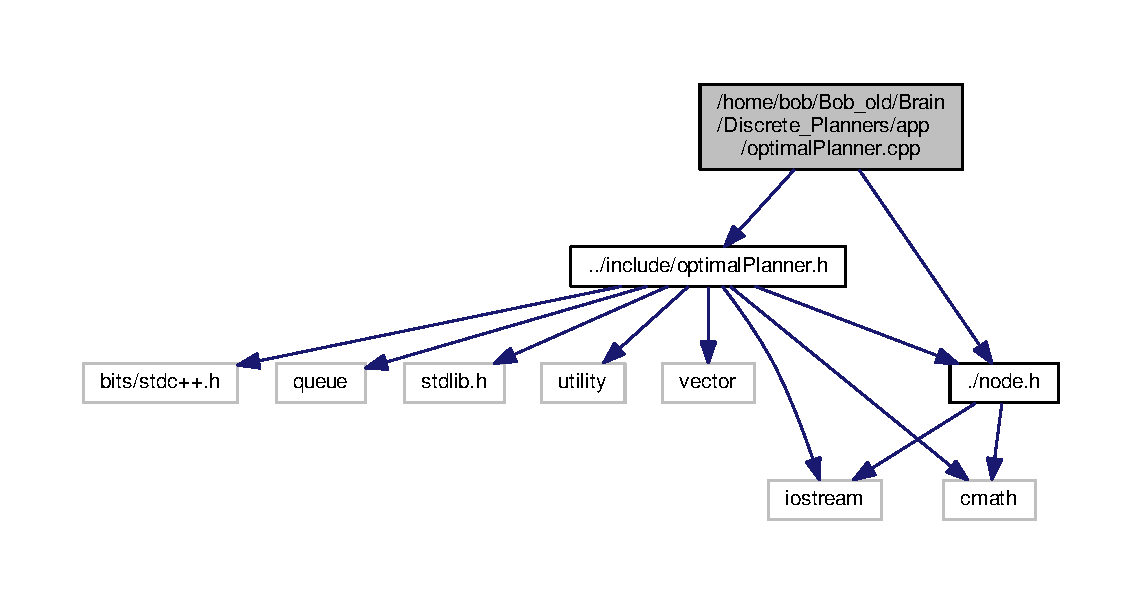
\includegraphics[width=350pt]{optimalPlanner_8cpp__incl}
\end{center}
\end{figure}


\subsection{Detailed Description}
Astar Algorithm A$\ast$ Search Algorithm\+: At each step it picks the node according to a value-\/‘f’ which is a parameter equal to the sum of two other parameters – ‘g’ and ‘h’. At each step it picks the node/cell having the lowest ‘f’, and process that node/cell. g cost = the movement cost to move from the starting point to a given node on the grid, following the path generated to get there. h cost = the estimated movement cost to move from that given node on the grid to the final destination. 

Here we are using Manhattan Distance for calculating h cost for each nodes

Working\+:
\begin{DoxyEnumerate}
\item Add the starting node (or node) to the open list.
\item Repeat the following\+:
\end{DoxyEnumerate}

A) Look for the lowest F cost node on the open list. We refer to this as the current node.

B). Switch it to the closed list.

C) For each of the 4 nodes adjacent to this current node …

If it is not walkable or if it is on the closed list, ignore it. Otherwise do the following. If it isn’t on the open list, add it to the open list. Make the current node the parent of this node. Record the F, G, and H costs of the node. If it is on the open list already, check to see if this path to that node is better, using G cost as the measure. A lower G cost means that this is a better path. If so, change the parent of the node to the current node, and recalculate the G and F scores of the node. If you are keeping your open list sorted by F score, you may need to resort the list to account for the change. D) Stop when you\+:

Add the target node to the closed list, in which case the path has been found, or Fail to find the target node, and the open list is empty. In this case, there is no path.
\begin{DoxyEnumerate}
\item Save the path. Working backwards from the target node, go from each node to its parent node until you reach the starting node. That is your path.

\begin{DoxyAuthor}{Author}
Bhargav Dandamudi 
\end{DoxyAuthor}
\begin{DoxyVersion}{Version}
1 
\end{DoxyVersion}
\begin{DoxyDate}{Date}
2019-\/04-\/04 
\end{DoxyDate}

\end{DoxyEnumerate}